测试pgf图片

% preamble:
\pgfplotsset{compat=1.3,compat/path replacement=1.5.1} 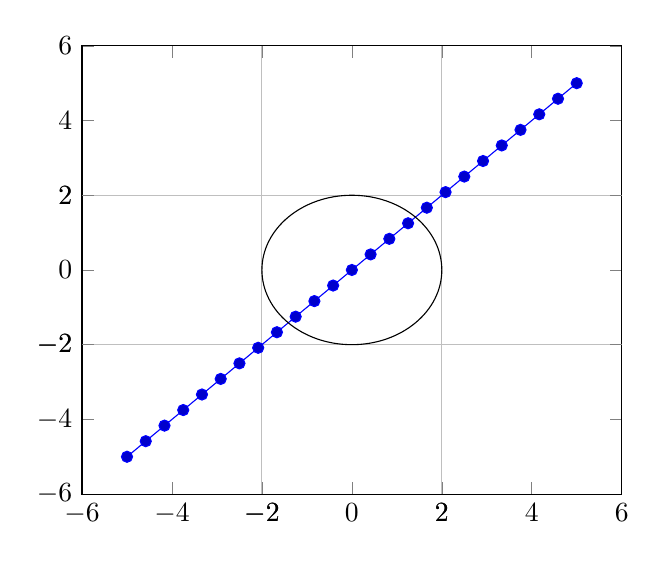
\begin{tikzpicture}
\begin{axis}[
extra x ticks={-2,2},
extra y ticks={-2,2},
extra tick style={grid=major}] \addplot {x};
\draw (axis cs:0,0) circle[radius=2];
\end{axis}
\end{tikzpicture}

\begin{tikzpicture}
\node[place, label=center:A] (p1) {};
\node[place, right=of p1] (p2) {};
\end{tikzpicture}



\begin{tikzpicture}
\node[place, label=center:A]    (A)     at ( -2.5, 0 )     [circle,draw=blue!50,fill=blue!20]  {};
\node[place, label=center:B]    (B)     at ( -1,   2 )     [circle,draw=blue!50,fill=blue!20]  {}
    edge [-, red, ultra thick, bend right] (A);
\node[place, label=center:C]    (C)     at ( 1, 2    )     [circle,draw=blue!50,fill=blue!20]  {}
    edge [-, blue, ultra thick] (A)
    edge [-, blue, ultra thick] (B);
\node[place, label=center:D]    (D)     at ( 2.5, 0  )     [circle,draw=blue!50,fill=blue!20]  {}
    edge [-, red, ultra thick] (A)
    edge [-, red, ultra thick] (B)
    edge [-, blue, ultra thick, bend right] (C);
\node[place, label=center:E]    (E)     at ( 1, -2   )     [circle,draw=blue!50,fill=blue!20]  {}
    edge [-, blue, ultra thick] (A)
    edge [-, blue, ultra thick] (B)
    edge [-, red, ultra thick] (C)
    edge [-, blue, ultra thick, bend right] (D);
\node[place, label=center:F]    (F)     at ( -1, -2  )     [circle,draw=blue!50,fill=blue!20]  {}
    edge [-, blue, ultra thick, bend left] (A)
    edge [-, blue, ultra thick] (B)
    edge [-, red, ultra thick] (C)
    edge [-, red, ultra thick] (D)
    edge [-, red, ultra thick] (E);
\end{tikzpicture}
